\documentclass[conference]{main}
\IEEEoverridecommandlockouts
% The preceding line is only needed to identify funding in the first footnote. If that is unneeded, please comment it out.
\usepackage{cite}
\usepackage{amsmath,amssymb,amsfonts}
\usepackage{algorithmic}
\usepackage{graphicx}
\usepackage{textcomp}
\usepackage{xcolor}
\def\BibTeX{{\rm B\kern-.05em{\sc i\kern-.025em b}\kern-.08em
    T\kern-.1667em\lower.7ex\hbox{E}\kern-.125emX}}
\begin{document}

\title{
    Development of an IoT-Based Virtual Fencing System with Advanced Monitoring and
    Animal Tracking Capabilities\\
{\footnotesize Engineering Project Design - EGD107V }
% \thanks{Identify applicable funding agency here. If none, delete this.}
}

\author{
\IEEEauthorblockN{1\textsuperscript{st} Otsile Earl Kole}
\IEEEauthorblockA{\textit{dept. Computer System Engineering} \\
Pretoria, South Africa\\
9701532@tut4life.ac.za}
\and
\IEEEauthorblockN{1\textsuperscript{st} Simanga H. Khoza}
\IEEEauthorblockA{\textit{dept. Computer System Engineering} \\
Pretoria, South Africa\\
214651459@tut4life.ac.za}
}

\maketitle

% \begin{abstract}
% In this section you include your abstract which is not more than 300 words. An
% abstract act like a 'mini' version of the paper and follows the same structure
% as the main text (that is discussed below). It contains 4Ps of a successful
% abstract (Problem, Purpose, Process and Possible outcomes. It contains: (i) an
% introduction to the topic (Problem and purpose); (ii) the main material, method
% and research design – used or used (Process); and (iii) mentions the
% recommendations/outcomes (Possible outcomes).
% \end{abstract}

% \begin{IEEEkeywords}
% component, formatting, style, styling, insert
% \end{IEEEkeywords}

\section{Introduction}
The global demand for beef continues to escalate alongside the expanding
population, underscoring the need for enhanced efficiency in beef production. To
meet this growing demand sustainably\cite{b1}, it is imperative to explore innovative
solutions that optimize livestock management practices. This paper introduces a
groundbreaking concept: a virtual fencing system empowered by IoT technology to
revolutionize the way farmers manage and monitor their cattle operations. While
various industries have already harnessed the benefits of data monitoring and
tracking technologies, the agricultural sector has been relatively slower in
adopting these advancements. By integrating real-time monitoring capabilities
into livestock management, farmers stand to benefit from reduced labor costs,
streamlined farm operations, and improved overall efficiency. This
transformative approach not only enhances day-to-day farm management but also
facilitates long-term planning, enabling farmers to make informed decisions and
optimize productivity on their busy farms.

\subsection{Define project problems}

Recent statistics indicate that stock theft has seen a marginal increase of
0.6\% in the third quarter of the 2022/23 financial year. Gauteng experienced
the largest increase of 39.8\%, followed by the Northern Cape with a 31.3\%
increase\cite{b1}. It’s also noted that a significant portion of stock theft cases go
unreported, with estimates suggesting that around 70.7\% of cases are not
reported\cite{b2}.

% IoT-based virtual fencing can assist in mitigating stock theft through
% real-time monitoring and tracking of livestock. This technology allows for the
% creation of geofences, which are virtual boundaries that can be adjusted as
% needed without physical barriers. When an animal approaches or crosses these
% boundaries, farmers can receive alerts. Additionally, IoT devices can track the
% health and behaviour of animals, providing valuable data that can be used to
% improve farm management and security\cite{b3}.

% By integrating IoT-based systems, farmers can enhance their ability to monitor
% livestock movements, detect unusual behaviour that may indicate theft, and
% respond promptly to secure their assets. This proactive approach to livestock
% management not only helps in preventing stock theft but also contributes to the
% overall well-being and productivity of the herd.

This project attempts to address several key problems in livestock management:

\begin{itemize}
    \item   Land Management: It allows for more efficient use of pastureland, as virtual fences can be easily moved to manage grazing patterns without the need for physical barriers\cite{b4}.
    \item   Environmental Impact: By controlling where livestock graze, it helps prevent overgrazing and land degradation, contributing to more sustainable farming practices\cite{b3}.
    \item   Labor Costs: Reduces the labor and resources required to build and maintain traditional fences, leading to cost savings for farmers \cite{b3}.
    \item   Animal Welfare: Enhances the well-being of animals by monitoring their health and behavior, allowing for timely intervention when necessary \cite{b4}.
    \item   Theft Prevention: Offers a solution to stock theft by providing real-time alerts when animals move outside of designated boundaries \cite{b3}.
\item   Data Collection: Collects valuable data on livestock, which can be used for improving breeding programs, tracking diseases, and making informed management decisions \cite{b4}.
\end{itemize}


\section{Literature}

\subsection{Similar Studies}

\begin{itemize}

\item   Virtual Fencing Technology for Cattle Management in the Pasture Feeding
    System \cite{b5}.
        The method of the above focuses on using virtual fencing technology to
        manage cattle for pasture feeding. The study further provides technical
        comparison of different systems that are currently on the market.
        Gap: The view of the study is that there still a need for an
        improvement that will decrease the cost and increase efficiency of the
        technology.

\item   Monitoring and controlling behaviors of livestock using virtual
    fences\cite{b6}.
    The method used in the above-mentioned study is that it uses sound and a
        electronic shocker in controlling the livestock. The paper outlines the
        intention of adding health information as their future work.
    Gap: The study failed to consider the health risk of the electric shocker and the behavioral change of the tools used.

\item   Monitoring Cattle Grazing Behavior and Intrusion Using Global
    Positioning System and Virtual Fencing\cite{b7}.

\item The study above used a different approach on also looking at what others have said about the use of global positioning system and virtual fencing. The authors improved on what others has already implemented. They further looked into the comparison of various IoT devices.

\item    Automated Virtual Fencing Can Effectively Contain Trials and Prospects\cite{b8}.
    The method of the study mainly focuses on the commercialized IoT devices
        that are mainly used in cattle. The focus of the study was to use sheep
        in order to determine how they will react towards the technology.
    Gap: The study was to put the commercialized technology into trial to see their effectiveness on sheep. It was concluded that the were effective however they still need an improvement when it comes to sheep than cattle.

\item Does Virtual Fencing Work for Grazing Dairy Cattle\cite{b9}?
\item The method of the study was to mainly demonstrate commercialized automated virtual fence collar on cattle. However, the study shows an extreme variation from one animal to another.

\end{itemize}


Gap:
To determine the impact of monitoring of the virtual fence and IoT device on require implementing it over a longer duration. However, the study only implemented it over a short period of time, which might impact the study's outcome.



\subsection{Virtual Fencing Techniques}

Extensive studies have delved into various methods of virtual fencing,
encompassing auditory, electrical, or combined stimuli to influence animal
behavior. These techniques are typically classified into static and dynamic
virtual fences, each characterized by distinct technical attributes, benefits,
and drawbacks.

\subsection{Animal Control and Behavior Modification}

Research findings have demonstrated the efficacy of virtual fencing in modifying
animal behavior, enabling improved management of free-range livestock. By
delivering sensory signals to animals when they approach electronically defined
boundaries, virtual fencing facilitates enhanced control and supervision of
livestock movements.

\subsection{Ecological and Economic Benefits}

The adoption of virtual fencing not only streamlines ecological management by
transitioning physical labor to cognitive tasks but also reduces the resource
and labor expenses associated with traditional fencing methods. Consequently,
virtual fencing offers substantial economic advantages to farmers and ranchers.

\subsection{Challenges and Limitations}

Despite its potential, virtual fencing presents challenges related to optimal
animal control, including concerns about animal stress, technology reliability,
and the necessity for further research to assess long-term effects on livestock
behavior and well-being.

In summary, the literature review highlights the evolution of virtual fencing
techniques, their impact on animal behavior modification, and the ecological and
economic benefits they offer. It also acknowledges the challenges and
limitations associated with virtual fencing, emphasizing the need for ongoing
research to optimize animal control practices. Furthermore, the integration of
IoT advancements in virtual fencing is explored, showcasing the expanded
capabilities of these systems in monitoring and managing livestock.


\section{Methodology}

\subsection{Challenges and Limitations}

A mixed-method research design will be employed for the development of an
IoT-Based Virtual Fencing System with Advanced Monitoring and Animal Tracking
Capabilities. This design will include quantitative data collection and
analysis, as well as qualitative research methods to gather insights from
farmers on how it affects the cattle. The project will utilize design thinking,
which emphasizes a human-centered approach to problem-solving and innovation.
The scientific and engineering process will involve conducting a thorough
literature review, designing and prototyping the virtual fencing system, testing
and refining the system through iterative feedback loops, and ultimately
evaluating its effectiveness in real-world settings. Additionally, the research
will involve collaboration with experts in IoT technology, animal behavior, and
agriculture to ensure the system meets the needs and requirements of its
intended users.

\subsection{System block diagram}

The IoT-based Virtual Fencing System with Advanced Monitoring and Animal
Tracking Capabilities will use modern web technologies like JavaScript, Node.js,
and HTML to create a user-friendly frontend interface. Real-time data
communication between the client and server will be enabled through a Web socket
server, ensuring smooth and efficient information exchange. Furthermore, the
system will utilize GPS location services from Azure Maps to accurately track
and monitor the movement of animals within the virtual fencing area. The diagram
below gives a detailed overview of the system architecture, showcasing how these
technologies are integrated for optimal performance and functionality.

\begin{figure}[htbp]
\centering
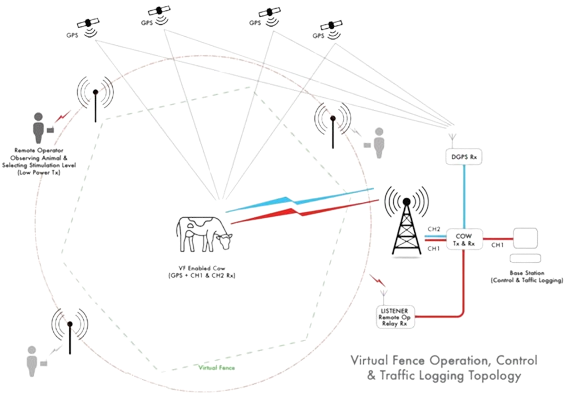
\includegraphics[width=\columnwidth]{system-removebg-preview.png}
\caption{System Overview}
\label{fig}
\end{figure}

\subsection{Tools Analysis}

A variety of tools and technologies will be utilized in the
development of the IoT-Based Virtual Fencing System with Advanced Monitoring and
Animal Tracking Capabilities. These tools include ESP32 development boards,
which will serve as the core hardware component for implementing the IoT
functionalities of the system. Additionally, GPS sensors and trackers will be
integrated to enable precise location tracking of animals within the virtual
fencing area. The use of a 3D printer will allow for the fabrication of custom
cases to house the electronic components securely.

Furthermore, a web server hosted online will provide the necessary
infrastructure for remote access and data storage, ensuring seamless
connectivity and accessibility for users. To interact with the system, users
will require a computer with internet access or a compatible web browser,
enabling them to monitor and manage the virtual fencing system from any
location. These research tools will be instrumental in the successful
development and deployment of the innovative IoT-based solution.

\subsection{Ethical Clearance, Health, and Safety}

One of the critical aspects is to ensure that the technology that is going to
be deployed adheres to the ethical guidelines and regulations. Furthermore, the
project should not cause any harm, distress, or discomfort.

In addition, the people or farmers who will be involved in the project when they
are installing or maintaining the system must always follow safety protocols.

Any data collected from animals or farm workers will be handled securely and
confidentially.


\section{Expected Outputs}

The calculated engineering output for the system will involve the implementation
of stimulus feedback mechanisms, such as sound or vibration signals, to be
transmitted to the IoT devices worn by the livestock when they cross the
boundaries set by the farmers. This feedback system will serve as a deterrent to
prevent animals from straying beyond the designated virtual fence perimeter.

To achieve this, sophisticated algorithms will be developed and integrated into
the system to accurately detect and analyze GPS coordinates in real-time. These
algorithms will be designed to effectively determine if a particular set of GPS
coordinates falls within the predefined boundaries of the virtual fence. By
leveraging advanced geofencing technology and precise location tracking
capabilities, the system will be able to trigger the appropriate feedback
response when livestock approach or breach the virtual fencing boundaries. This
innovative approach will enhance the overall effectiveness and efficiency of the
IoT-based virtual fencing system, ensuring optimal monitoring and control of
animal movement on the farm.



\subsection{Benefits to Society}

The implementation of this IoT-Based Virtual Fencing System with
Advanced Monitoring and Animal Tracking Capabilities will bring about numerous
benefits to society. One of the key advantages is the enhancement of food
security, as the system enables farmers to efficiently manage and monitor their
livestock, ensuring a consistent and reliable food supply. By leveraging
technology to streamline the farming process, farmers can produce higher yields
with reduced labor requirements, ultimately leading to increased productivity
and sustainability in food production.

Furthermore, the widespread adoption of this technology on a large scale has the
potential to positively impact the market dynamics of the agricultural industry.
By optimizing the management of livestock and reducing operational costs, the
system can contribute to driving down the price of beef and other livestock
products. This affordability can benefit consumers by making high-quality meat
products more accessible and affordable, while also supporting the economic
viability of farmers and ranchers. Overall, the societal benefits of this
innovative technology extend beyond the agricultural sector, offering a
sustainable and efficient solution for food production and resource management.

\begin{enumerate}

    \item \textbf{Enhanced Food Security:}
        \begin{itemize}
        \item   By enabling efficient management and monitoring of livestock, this system ensures a consistent and reliable food supply.
        \item   Leveraging technology streamlines farming processes, leading to higher yields with reduced labour requirements.
        \item   This contributes to increased productivity and sustainability in food production.
        \end{itemize}

    \item \textbf{Market Dynamics Transformation:}
        \begin{itemize}
        \item   Widespread adoption of this technology on a large scale can positively impact the agricultural industry.
        \item   Optimized livestock management and reduced operational costs can drive down the price of beef and other livestock products.
        \item   Consumers benefit from more accessible and affordable high-quality meat products.
        \item   Simultaneously, this supports the economic viability of farmers and ranchers.
        \end{itemize}

    \item \textbf{Beyond Agriculture:}
        \begin{itemize}
        \item   The societal benefits extend beyond the agricultural sector.
        \item   This innovative technology offers a sustainable and efficient solution for food production and resource management.
        \end{itemize}

\end{enumerate}


\subsection*{Study Limitations}

The project will be using IoT devices that might have accuracy challenges which
might affect the effectiveness of virtual fencing. The above will lead to
errors in boundary detections that might lead to the unintended animal crossing
the virtual line or false alarms.

IoT devices used for tracking and virtual fencing require power (batteries and
solar panels). Therefore, the IoT devices will be required to be regularly
maintained to ensure that they function properly.

Different animal species may exhibit varying responses to this project. What
works effectively on one animal may work differently to the other one.

Lastly the environmental factors must be considered when implementing this
project, for example weather conditions might have an impact on the performance
of the IoT device to be used.

\begin{thebibliography}{00}
\bibitem{b1}	A. Coleman. "Stock theft statistics do not paint a true picture of the crime in SA." https://www.farmersweekly.co.za/agri-news/south-africa/stock-theft-statistics-do-not-paint-a-true-picture-of-the-crime-in-sa/ (accessed.
\bibitem{b2}	J. d. Klerk. "The impact of stock theft." saai.org. https://saai.org/en/the-impact-of-stock-theft/ (accessed.
\bibitem{b3}	M. Abdouna, D. Ahmat, and T. F. Bissyandé, "Virtual Fences: A Systematic Literature Review," Cham, 2023: Springer Nature Switzerland, in Towards new e-Infrastructure and e-Services for Developing Countries, pp. 115-148.
\bibitem{b4}	K. C. Reddy, S. K. R, S. Sharma, N. Gobi, S. D, and P. V. Prasanth, "Real-Time Tracking of Wildlife with IoT Solutions in Movement Ecology," Journal Of Advanced Zoology, vol. 44(S-3), pp. 1122-1134, October 2023 2023, doi: 10.17762/jaz.v44iS-5.1191.
\bibitem{b5}	P. Goliński, P. Sobolewska, B. Stefańska, and B. Golińska, "Virtual fencing technology for cattle management in the pasture feeding system—A review," Agriculture, vol. 13, no. 1, p. 91, 2022.
\bibitem{b6}	A. Muminov, D. Na, C. Lee, H. Kang, and H. S. Jeon, "Monitoring and controlling behaviors of livestock using virtual fences," J. Theor. Appl. Inf. Technol, vol. 97, no. 18, pp. 1-12, 2019.
\bibitem{b7}	R. W. Bello and O. M. Moradeyo, "Monitoring cattle grazing behavior and intrusion using global positioning system and virtual fencing," Asian Journal of Mathematical Sciences, 2019.
\bibitem{b8}	D. L. Campbell et al., "Automated virtual fencing can effectively contain sheep: field trials and prospects," Animals, vol. 13, no. 4, p. 619, 2023.
\bibitem{b9}	S. Lomax, P. Colusso, and C. E. F. Clark, "Does Virtual Fencing Work for Grazing Dairy Cattle?," Animals, vol. 9, no. 7, p. 429, 2019. [Online]. Available: https://www.mdpi.com/2076-2615/9/7/429.
\end{thebibliography}



% \subsection{Units}
% \begin{itemize}
% \item Use either SI (MKS) or CGS as primary units. (SI units are encouraged.) English units may be used as secondary units (in parentheses). An exception would be the use of English units as identifiers in trade, such as ``3.5-inch disk drive''.
% \item Avoid combining SI and CGS units, such as current in amperes and magnetic field in oersteds. This often leads to confusion because equations do not balance dimensionally. If you must use mixed units, clearly state the units for each quantity that you use in an equation.
% \item Do not mix complete spellings and abbreviations of units: ``Wb/m\textsuperscript{2}'' or ``webers per square meter'', not ``webers/m\textsuperscript{2}''. Spell out units when they appear in text: ``. . . a few henries'', not ``. . . a few H''.
% \item Use a zero before decimal points: ``0.25'', not ``.25''. Use ``cm\textsuperscript{3}'', not ``cc''.)
% \end{itemize}

% \subsection{Equations}
% Number equations consecutively. To make your
% equations more compact, you may use the solidus (~/~), the exp function, or
% appropriate exponents. Italicize Roman symbols for quantities and variables,
% but not Greek symbols. Use a long dash rather than a hyphen for a minus
% sign. Punctuate equations with commas or periods when they are part of a
% sentence, as in:
% \begin{equation}
% a+b=\gamma\label{eq}
% \end{equation}

% Be sure that the
% symbols in your equation have been defined before or immediately following
% the equation. Use ``\eqref{eq}'', not ``Eq.~\eqref{eq}'' or ``equation \eqref{eq}'', except at
% the beginning of a sentence: ``Equation \eqref{eq} is . . .''

% \subsection{Figures and Tables}
% \paragraph{Positioning Figures and Tables} Place figures and tables at the top and
% bottom of columns. Avoid placing them in the middle of columns. Large
% figures and tables may span across both columns. Figure captions should be
% below the figures; table heads should appear above the tables. Insert
% figures and tables after they are cited in the text. Use the abbreviation
% ``Fig.~\ref{fig}'', even at the beginning of a sentence.

% \begin{table}[htbp]
% \caption{Table Type Styles}
% \begin{center}
% \begin{tabular}{|c|c|c|c|}
% \hline
% \textbf{Table}&\multicolumn{3}{|c|}{\textbf{Table Column Head}} \\
% \cline{2-4}
% \textbf{Head} & \textbf{\textit{Table column subhead}}& \textbf{\textit{Subhead}}& \textbf{\textit{Subhead}} \\
% \hline
% copy& More table copy$^{\mathrm{a}}$& &  \\
% \hline
% \multicolumn{4}{l}{$^{\mathrm{a}}$Sample of a Table footnote.}
% \end{tabular}
% \label{tab1}
% \end{center}
% \end{table}



\end{document}
